% Source: Notion page “4. 数据处理与骨架特征构建”. Generated without rewriting its content.
\chapter{数据处理与骨架特征构建}

本系统采用基于人体骨架的行为识别方案。原始视频首先经过视频解码和时序采样，再使用经过 INT8 量化的RTMDet-S INT8 和 RTMPose-S 模型分别进行人体检测和关键点提取。针对校园交互行为中常见的双人场景，系统进一步通过时序轨迹关联保持人物身份的一致性，并最终形成统一的 COCO17 Skeleton Sequence，供后续轻量级行为识别模型使用。

整体数据预处理流程（RGB流）

\begin{figure}[htbp]
\centering
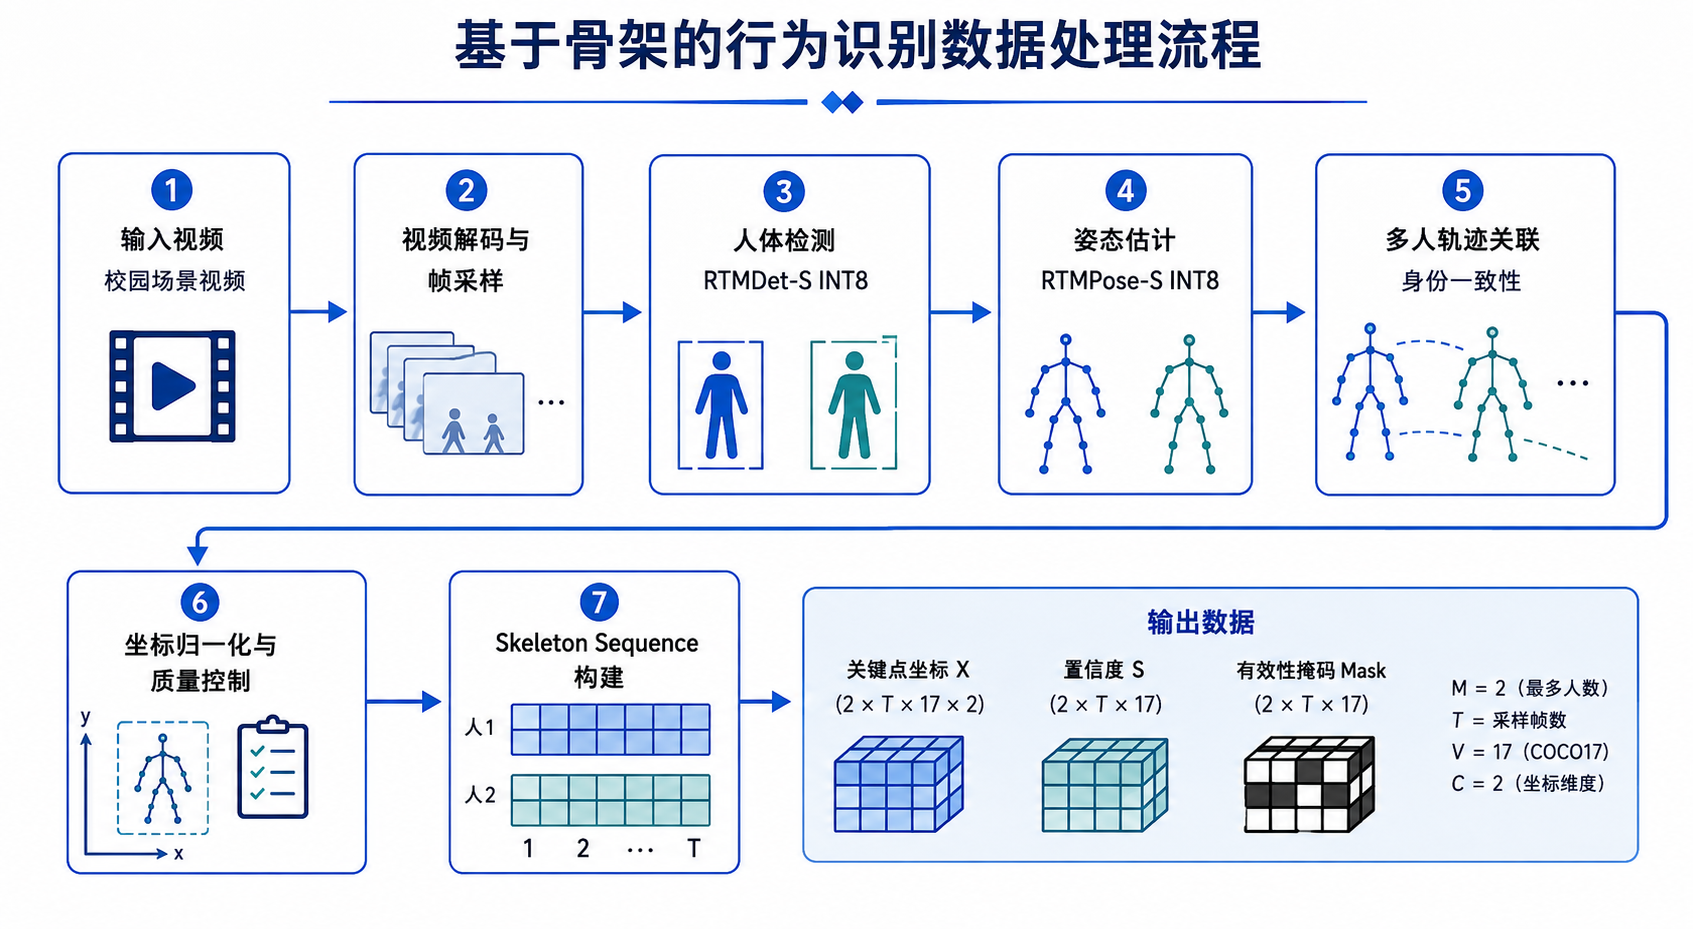
\includegraphics[width=0.96\linewidth,keepaspectratio]{figures/notion_image_02.png}
\end{figure}

\section{数据输入}

系统输入为校园场景视频：

\[
\mathcal{V}=\{I_0,I_1,\ldots,I_{N-1}\}
\]

其中，\(I_i\) 表示第 \(i\) 帧图像，\(N\) 表示视频总帧数，原始视频帧率记为 \(f_s\)，图像宽、高分别为 WW 和 HH。

系统支持 MP4、AVI 等常见视频格式。视频读取阶段主要检查视频是否可以正常打开、是否存在可解码帧，以及 FPS、分辨率等基本信息是否有效。

当视频无法提供有效帧率时，可采用默认帧率：

\[
f_s=30\ \text{FPS}
\]

以保证后续时序处理正常进行。

\section{视频帧处理}

\subsection{帧采样}

为降低姿态估计计算开销，同时尽可能保留完整动作过程，系统对原始视频进行时序采样。

设最大采样帧数为 \(T_{\max}\)。当：

\[
N\leq T_{\max}
\]

时，保留全部有效帧；当：

\[
N>T_{\max}
\]

时，在整个视频范围内进行均匀采样。

第 \(k\) 个采样帧位置为：

\[
i_k=
\operatorname{round}
\left(
\frac{k(N-1)}{T_{\max}-1}
\right),
\quad
k=0,1,\ldots,T_{\max}-1
\]

这种方法能够使采样帧覆盖动作的开始、发展和结束阶段，避免仅截取视频局部片段。

系统同时支持帧间隔参数 ss，仅处理满足：

\[
i\bmod s=0
\]

的帧。实时推理场景下通常设置：

\[
s=1
\]

即逐帧执行姿态估计。

\subsection{图像预处理}

采样得到的第 \(t\) 帧表示为：

\[
I_t\in\mathbb{R}^{H\times W\times3}
\]

图像直接送入人体检测与 RTMPose 推理流水线。模型所需的尺寸调整、归一化和 Tensor 转换由姿态估计推理框架统一完成。

\section{人体检测与多人姿态估计}

本系统采用 RTMDet-S + RTMPose-S 组成轻量级 Top-down 人体姿态估计流水线。

其中，RTMDet-S 负责在视频帧中定位人体，RTMPose-S 负责在检测到的人体区域中进一步预测人体关键点。

整体过程可表示为：

\[
I_t
\xrightarrow{\text{RTMDet-S}}
B_t^m
\xrightarrow{\text{RTMPose-S}}
P_t^m
\]

其中：

\begin{itemize}
\item \(I_t\)：第 \(t\) 帧图像；
\item \(B_t^m\)：第  帧中第  个人的人体检测框；
\item \(P_t^m\)：该人体对应的 COCO17 骨架关键点。
\end{itemize}

两个模型均采用 INT8 量化，以降低边缘侧推理的模型存储空间和计算开销。

\subsection{RTMDet-S 人体检测}

对于采样得到的第 \(t\) 帧图像：

\[
I_t\in\mathbb{R}^{H\times W\times3}
\]

首先使用 RTMDet-S 完成人体检测。

RTMDet-S 输出当前图像中的候选人体边界框集合：

\[
D_t=
\left\{
B_t^1,B_t^2,\ldots,B_t^K
\right\}
\]

其中，第 \(m\) 个检测结果表示为：

\[
B_t^m=
(x_1,y_1,x_2,y_2,s_{\text{det}})
\]

其中：

\begin{itemize}
\item \(x_1\),\(y_1\)：人体框左上角坐标；
\item \(x_2\),\(y_2\)：人体框右下角坐标；
\item \(s_{\text{det}}\)：人体检测置信度。
\end{itemize}

系统设置人体检测置信度阈值：

\[
x=0.15\tau_{\text{bbox}}=0.15
\]

仅保留满足：

\[
s_{\text{det}}\geq\tau_{\text{bbox}}
\]

的人体候选框。

随后采用非极大值抑制（Non-Maximum Suppression，NMS）去除高度重叠的重复人体框。NMS 的 IoU 阈值设置为：

\[
S=0.5\tau_{\text{NMS}}=0.5
\]

经过置信度过滤和 NMS 后，得到最终有效人体检测框，并送入 RTMPose-S 进行关键点估计。

因此，该阶段完成：

\[
I_t
\rightarrow
\{B_t^1,B_t^2,\ldots,B_t^K\}
\]

即从完整视频帧中确定“人体位于什么位置”。

\subsection{RTMPose-S 姿态估计}

对于 RTMDet-S 检测到的每一个有效人体框 \(B_t^m\)，系统截取或映射对应人体区域，并输入 RTMPose-S 进行二维姿态估计。

对于第 \(t\) 帧中的第 \(m\) 个人，RTMPose-S 输出：

\[
P_t^m=
\left\{
p_{t,1}^m,
p_{t,2}^m,
\ldots,
p_{t,17}^m
\right\}
\]

其中，第 \(j\) 个关键点表示为：

\[
p_{t,j}^m=
(x_{t,j}^m,y_{t,j}^m,s_{t,j}^m)
\]

其中：

\begin{itemize}
\item \(x_{t,j}^m\)：第 \(j\) 个关节点的横坐标；
\item \(y_{t,j}^m\)：第 \(j\) 个关节点的纵坐标；
\item \(s_{t,j}^m\)：该关节点的预测置信度。
\end{itemize}

因此 RTMPose-S 完成：

\[
\boxed{
(I_t,B_t^m)
\rightarrow
P_t^m
}
\]

即在 RTMDet-S 已确定人体位置的基础上，进一步判断“人体各关节位于什么位置”。

RTMDet-S 和 RTMPose-S 的功能分工如下：

\begin{center}
\small
\begin{longtable}{|>{\raggedright\arraybackslash}p{0.22\linewidth}|>{\raggedright\arraybackslash}p{0.22\linewidth}|>{\raggedright\arraybackslash}p{0.22\linewidth}|>{\raggedright\arraybackslash}p{0.22\linewidth}|}
\hline
模型 & 主要功能 & 输入 & 输出 \\
\hline
RTMDet-S INT8 & 人体检测与定位 & 视频帧 & Person Bounding Boxes \\
\hline
RTMPose-S INT8 & 人体姿态估计 & 人体区域 & COCO17 Keypoints \\
\hline
\end{longtable}
\end{center}

\subsection{COCO17 骨架关键点}

RTMPose-S 最终输出标准 COCO17 二维人体骨架，共包含 17 个关键点。

\begin{center}
\small
\begin{longtable}{|>{\raggedright\arraybackslash}p{0.22\linewidth}|>{\raggedright\arraybackslash}p{0.22\linewidth}|>{\raggedright\arraybackslash}p{0.22\linewidth}|>{\raggedright\arraybackslash}p{0.22\linewidth}|}
\hline
编号 & 英文名称 & 中文名称 & 人体区域 \\
\hline
0 & Nose & 鼻子 & 头部 \\
\hline
1 & Left Eye & 左眼 & 头部 \\
\hline
2 & Right Eye & 右眼 & 头部 \\
\hline
3 & Left Ear & 左耳 & 头部 \\
\hline
4 & Right Ear & 右耳 & 头部 \\
\hline
5 & Left Shoulder & 左肩 & 上肢 / 躯干 \\
\hline
6 & Right Shoulder & 右肩 & 上肢 / 躯干 \\
\hline
7 & Left Elbow & 左肘 & 上肢 \\
\hline
8 & Right Elbow & 右肘 & 上肢 \\
\hline
9 & Left Wrist & 左手腕 & 上肢 \\
\hline
10 & Right Wrist & 右手腕 & 上肢 \\
\hline
11 & Left Hip & 左髋 & 躯干 / 下肢 \\
\hline
12 & Right Hip & 右髋 & 躯干 / 下肢 \\
\hline
13 & Left Knee & 左膝 & 下肢 \\
\hline
14 & Right Knee & 右膝 & 下肢 \\
\hline
15 & Left Ankle & 左脚踝 & 下肢 \\
\hline
16 & Right Ankle & 右脚踝 & 下肢 \\
\hline
\end{longtable}
\end{center}

COCO17 骨架覆盖人体头部、躯干、双臂和双腿等主要结构。其中，肩部、肘部和手腕关键点可以反映挥手、推搡等上肢动作；髋部、膝部和脚踝关键点可以描述行走、奔跑、追逐等下肢运动；不同人物之间关键点位置随时间的变化还可以进一步反映双方接近、远离及身体交互等行为特征。

因此，COCO17 能够以较低的数据维度保留校园行为识别所需的主要人体运动信息。

\section{人体关联与跟踪}

单帧姿态估计只能判断当前帧中存在的人体，而行为识别需要保证同一人物在连续帧中的身份一致。因此，本系统采用基于 Bounding Box IoU 与中心距离 的轻量级贪心跟踪算法进行跨帧人物关联。

\subsection{IoU 匹配}

设历史轨迹框为 BtrackB\textasciicircum{}\{track\}，当前检测框为 BdetB\textasciicircum{}\{det\}，两者的交并比定义为：

\[
\frac{
|B^{track}\cap B^{det}|
}{
|B^{track}\cup B^{det}|
}
\]

IoU 越大，说明两个检测框在空间位置上越接近。

\subsection{中心距离}

考虑到快速运动时相邻帧的人体框可能重叠较少，系统同时计算归一化中心距离。

人体框中心定义为：

\[
\left(
\frac{x_1+x_2}{2},
\frac{y_1+y_2}{2}
\right)
\]

归一化中心距离定义为：

\[
d=
\frac{
\|c(B^{track})-c(B^{det})\|_2
}{
\max(
diag(B^{track}),
diag(B^{det}),
1
)
}
\]

其中 diag(B)diag(B) 表示人体框对角线长度。

当满足：

\[
IoU\geq0.05
\]

或：

\[
d\leq0.55
\]

时，将该检测视为历史轨迹的候选匹配。

候选匹配得分定义为：

\[
e_{match}=IoU-0.15d
\]

系统按照匹配得分从高到低进行贪心分配，并保证一个检测框只能对应一条轨迹。

\subsection{短时遮挡处理}

校园场景中可能出现人体遮挡或短时间漏检，因此系统允许轨迹短时间失去观测。

设当前帧与轨迹最后出现帧之间的间隔为：

\[
\Delta t=t-t_{last}
\]

当：

\[
\Delta t\leq G_{\max}
\]

时，该轨迹仍然参与后续匹配。

系统采用：

\[
G_{\max}=6s
\]

其中 ss 为帧采样间隔。

\subsection{双人轨迹选择}

由于视频中可能存在背景行人，本系统不直接采用最先检测到的两个人，而根据轨迹持续时间、检测置信度和人体框大小进行排序。

第 \(m\) 条轨迹的评分定义为：

\[
R_m=
N_m\cdot\bar{s}_m
\cdot
\left(
1+
\frac{
\sqrt{\operatorname{median}(A_m)}
}{1000}
\right)
\]

其中：

\begin{itemize}
\item \(N_m\)：该轨迹的有效观测帧数；
\item \(\bar{s}_m\)：平均人体检测置信度；
\item \(A_m\)：轨迹对应的人体框面积。
\end{itemize}

最终选取得分最高的两条轨迹：

\[
M\leq2
\]

作为后续行为识别的主要人物。

\section{坐标归一化}

RTMPose 原始输出为图像像素坐标 (x,y)(x,y)。为了消除不同视频分辨率带来的影响，将坐标归一化至 [0,1][0,1] 范围。

对于图像宽度 WW 和高度 HH：

\[
\tilde{x}=\frac{x}{W}
\]

\[
\tilde{y}=\frac{y}{H}
\]

因此每一个关键点表示为：

\[
\tilde{p}_{t,j}^{m}
=
(\tilde{x}_{t,j}^{m},
\tilde{y}_{t,j}^{m})
\]

经过归一化后，不同分辨率的视频均具有统一的坐标尺度，便于后续模型进行时空特征学习。

\section{时序质量控制与关键点处理}

\subsection{关键点置信度过滤}

RTMPose 为每一个关键点输出置信度：

\[
s_{t,j}^{m}\in[0,1]
\]

系统设置关键点有效阈值：

\[
\tau_{kp}=0.20
\]

定义有效性掩码：

\[
Mask_{t,j}^{m}
=
\begin{cases}
1,&s_{t,j}^{m}\geq\tau_{kp}\\
0,&s_{t,j}^{m}<\tau_{kp}
\end{cases}
\]

最终得到：

\[
\in\{0,1\}^{M\times T\times17}
\]

低置信度关键点不会导致整帧被删除，而是通过 Mask 标记其有效性，从而尽量保留其他可靠人体关节信息。

\subsection{人体缺失处理}

当某一帧中某一人物未被检测到时，系统保持原有时间位置，并将对应骨架坐标和关键点置信度置零：

\[
X_{m,t,:,:}=0
\]

\[
S_{m,t,:}=0
\]

这样可以保持时间序列结构完整，并避免因直接删除帧而破坏动作时序关系。

\subsection{时序平滑与插值}

当前主推理链路不过度使用时序平滑，因为推搡、挥手和快速追逐等行为本身包含较明显的高频运动信息，过强滤波可能削弱有效动作特征。

系统主要依赖：

关键点置信度 + 人体跟踪 + 有效性 Mask

完成质量控制。

对于少量连续缺失的关键点，可选用线性插值。若关键点在 \(t_a\) 与 \(t_b\) 时刻有效，则中间位置可表示为：

\[
\frac{t-t_a}{t_b-t_a}
(P_{t_b}-P_{t_a}),
\quad
t_a<t<t_b
\]

仅对较短缺失区间进行插值，较长时间缺失仍保持无效状态，以避免人为生成错误运动轨迹。

\section{输出格式}

当前系统直接保留 RTMPose 输出的 COCO17 二维骨架表示。最终单个视频的骨架数据表示为：

\[
X\in\mathbb{R}^{M\times T\times V\times C}
\]

其中：

\begin{itemize}
\item M：最多保留的人数，本系统取 M=2；
\item T：视频经过采样后的帧数；
\item V：人体关键点数量，COCO 格式下 V=17；
\item C：关键点坐标维度，本系统采用二维坐标，因此 C=2。
\end{itemize}

另外保存关键点置信度：

\[
S\in\mathbb{R}^{M\times T\times V}
\]

用于表示每一个关键点的检测可信程度。

以及关键点有效性掩码：

\[
\in\{0,1\}^{2\times T\times17}
\]

其中：

\[
\mathrm{Mask}_{m,t,j}=[S_{m,t,j}\geq 0.20]
\]

